\section{Outputs:}
The code returns us a matrix $[x\, y\, width\, height]$ with a dimension of $n\times 4$ of the detected objects such that:
\begin{itemize}
	\item $n$: Number of objects detected.
	\item $x$: Coordinate of the row, where the object in the image begins.
	\item $y$: Coordinate of the column, where the object in the image begins. %
	\item $width$: Width of the detected object.
	\item $height$: Height of the detected object.
\end{itemize}
We will call each row of this matrix \textbf{Rectangle} $Rectangle^{i}$. In figure \ref{fig:rect} we can see the example of a $Rectangle^{i}$ matrix within an image.
\begin{figure}[h!]
	\centering
	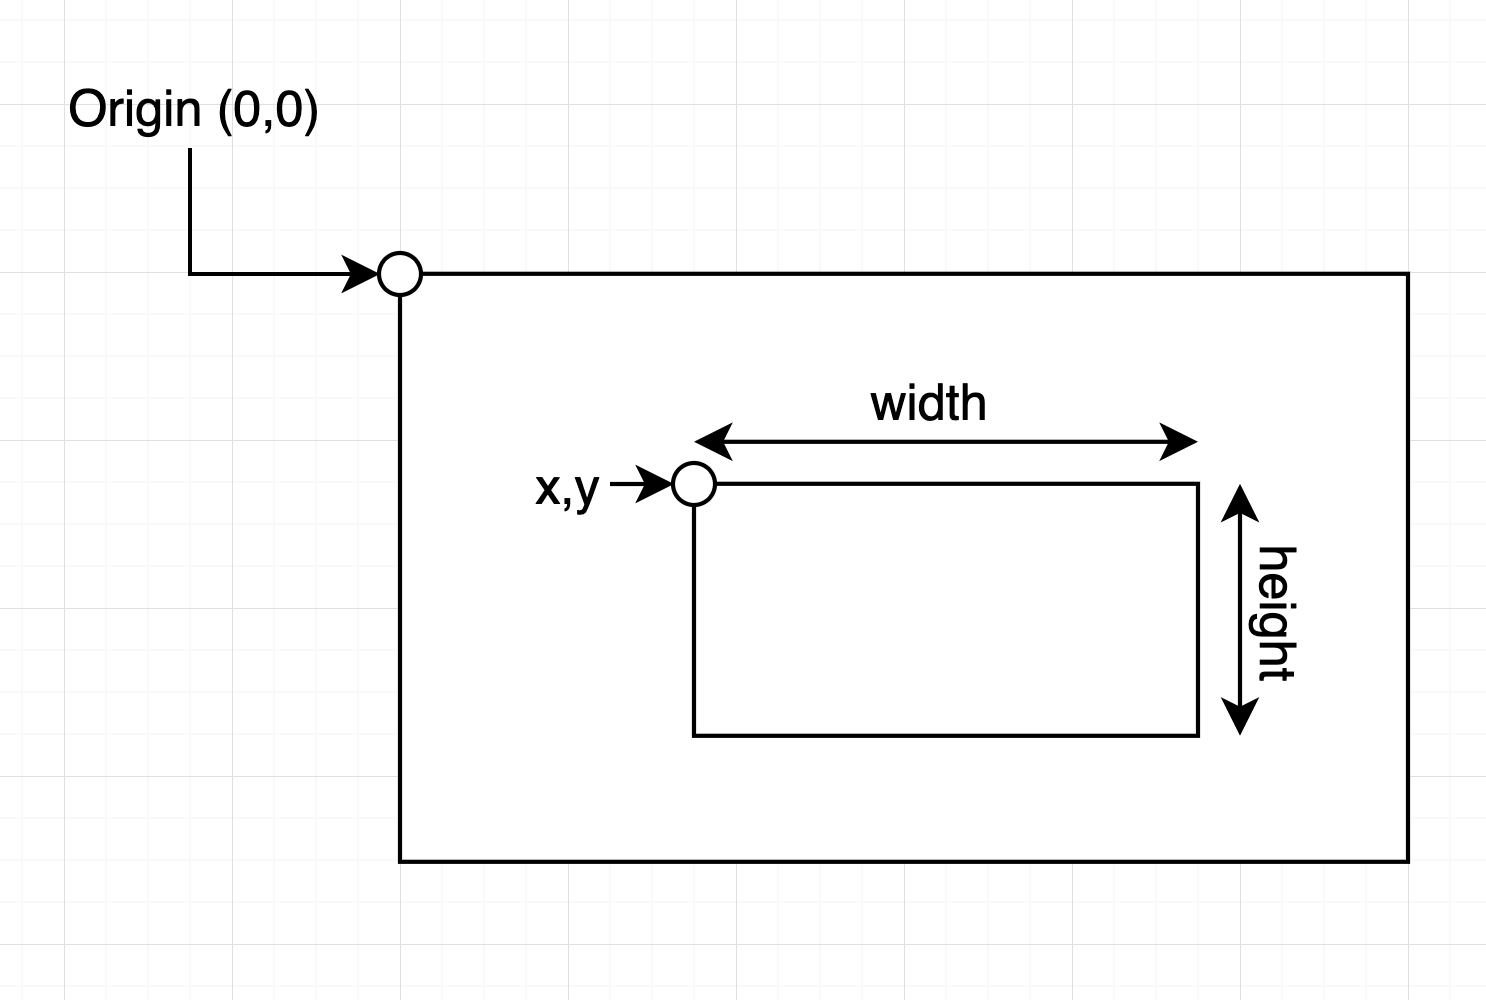
\includegraphics[scale=0.3]{T1/rectangle}
	\caption{$Rectangle^{i}$ matrix.}
	\label{fig:rect}
\end{figure}